\chapter{研究方法介绍}
张量决策图(TDD)是一种基于张量网络,结合了二元决策图的表示优势的数据结构。
TDD针对于量子计算,可以有很好的空间优势,同时也可以很方便的结合过去在二元决策图的模型检测算法的优化技术。
本章将主要介绍在本次研究中使用的方法,因此将主要介绍TDD和进一步的改进方案,并与类似技术进行对比,然后介绍如何应用TDD进行模型检测,最后介绍本次研究中的软件实现。
\section{TDD介绍}
TDDs是一种决策图样式的数据结构,用于使用张量网络表示量子电路。
本节将从用张量网络表示量子电路开始,然后简单介绍张量网络如何转换到TDD,最后介绍TDD之间的运算。
\subsection{张量网络表示量子线路}
张量是与一组与索引序列\(I=\{x_1,\ldots,x_n\}\)相关联的多维线性映射。在量子计算中,可以假设只从\(\{0,1\}\)中取值。因此,张量定义为定义\ref{df-tensor}所示。
\begin{definition}
    \label{df-tensor}
    当张量只从从\(\{0,1\}\)中取值时,对于定义在索引序列\(I\)上的张量\(\phi\),其可以表示为一个字典
    \begin{align}
        \phi :{\{0,1\}}^I\rightarrow\mathbb{C}
    \end{align}
    其中\(\mathbb{C}\)为复数。
\end{definition}


一个向量表示为$[\alpha_0,\alpha_1]$的量子比特x可以描述为秩为1的张量$\phi_x$,其中$\phi_x\left(0\right)=\alpha_0, \phi_x\left(1\right)=\alpha_1$。具有输入比特x和输出比特y的单比特门可以表示为秩为2的张量$\phi_{xy}$。类似的$n$比特量子门可以表示成一个秩为$2n$的张量。在张量表示中,一般不区分输入和输出索引。只有当将张量解释为门或电路时会规定关于其信息。
\begin{example}
    以单比特门Z门为例,其矩阵形式如式子\ref{eq-pauli}。当以x作为输入比特索引和y作为输出比特索引时,Z门的张量表示如式子\ref{eq-tensor-z}所示。
    \begin{align}
        \label{eq-tensor-z}
        \phi_{xy}\left(00\right)=1,\phi_{xy}\left(01\right)=0,\phi_{xy}\left(10\right)=0,\phi_{xy}\left(11\right)=-1
    \end{align}
\end{example}

张量之间最重要的运算之一是收缩(contraction)。收缩是通过对共享索引求和获得新的张量。具体来说,设 张量$\gamma_{\overrightarrow{x},\overrightarrow{z}}$ 和 $\xi_{\overrightarrow{y},\overrightarrow{z}}$ 的共享索引集 是$\overrightarrow{z}$。设收缩后的新张量为 $\phi_{\overrightarrow{x},\overrightarrow{y}}$,则其表达式如式子\ref{eq-contraction}所示。
\begin{equation}
\label{eq-contraction}
\phi_{\overrightarrow{x},\overrightarrow{y}}(\overrightarrow{a},\overrightarrow{b}) = \sum_{\overrightarrow{c} \in \{0,1\}^{\overrightarrow{z}}} \gamma_{\overrightarrow{x},\overrightarrow{z}}(\overrightarrow{a}, \overrightarrow{c}) \cdot \xi_{\overrightarrow{y},\overrightarrow{z}}(\overrightarrow{b}, \overrightarrow{c}).
\end{equation}

另一个重要的张量操作是切片(slicing),它对应于布尔函数的余因子运算。设 $\phi$ 是索引序列为 $I$ 上的张量。任取一个索引\(x\in I\),对 $\phi$ 进行关于 $x = c$ 与 $c \in \{0, 1\}$ 的切片也是一个张量 $\phi|_{x=c}$,在索引集 $I' =I/\{x\}$ 上定义如式子\ref{eq-slicing}所示。
\begin{equation}
    \label{eq-slicing}
\phi|_{x=c}(\overrightarrow{a}) := \phi(c, \overrightarrow{a})
\end{equation}
对于任意 $\overrightarrow{a} \in \{0, 1\}^n$。称 $\phi|_{x=0}$ 和 $\phi|_{x=1}$ 分别为 $\phi$ 关于 $x$ 的负切片(negative slicing)和正切片(positive slicing)。如果 $\phi|_{x=0} \neq \phi|_{x=1}$,称索引 $x \in I$ 对于 $\phi$ 是本质的(essential)。同时张量满足定理\ref{lemma-tensor}中的性质。

\begin{lemma}
    \label{lemma-tensor}
    对于定义在索引序列\(I\)上的张量\(\phi\),其中的每个索引\(x\in I\),都有
    \begin{align}
        \phi = \bar{x}\cdot \phi|_{x=0}+x\cdot \phi|_{x=1}
    \end{align}
\end{lemma}

张量网络是一个无向图\(G=\left(V,E\right)\)。其中顶点集$V$中的每个顶点$v$表示一个张量。边集\(E\)中每条边\(e\)代表与相邻两个张量相关联的公共索引。通过以任意顺序收缩连接的张量,可以得到一个秩为\(m\)的张量,其中\(m\)是$G$中开放边数。这个独立于收缩顺序的张量也称为该张量网络的张量表示\citep{biamonte2019lectures}。
张量网络提供了一种新的量子线路表示方法\citep{pednault2017breaking}。而当给定量子线路中所有量子门的输入和输出状态的索引值,收缩掉共享的索引,就可以得到量子电路的张量表示。
\begin{example}
    \label{ex-tensor}
    以图\ref{fig:example_cir_2}中的量子线路为例,线路中包含$T$和$H$两个不同的单比特门,以及一个两比特的受控非门$CX$。
式子\ref{eq-hardmard},\ref{eq-t},\ref{eq-cx}分别给出了$H,T,CX$门的矩阵形式,可以看到$T$门是一个对角门,即$T$门不改变输入态,而是根据输入态作用一个相位。同时$CX$不改变控制比特。因此可以只用索引$x_0$表示第一个比特。
图\ref{fig:example_cir_map}给出了图\ref{fig:example_cir_2}中量子线路中各个状态的索引值,从而可得的张量表示:
\begin{align}
\label{eq-tensor}
\phi_{x_0x_0y_0y_3}\left(a_0a_0b_0b_3\right)=\sum_{b_1,b_2=0}^{1}T\left(a_0a_0\right)H\left(b_0b_1\right)CX\left(a_0a_0b_1b_2\right)T\left(a_0a_0\right)H\left(b_2b_3\right)
    \end{align}
\begin{figure}[!htbp]
    \centering
    \includegraphics[width=.6\textwidth]{Img/example_cir_2.pdf}
    \caption{一个量子线路示例,是图\ref{fig:example_cir_map}表示的量子线路}   
    \label{fig:example_cir_2}
\end{figure}
\begin{figure}[!htbp]
    \centering
    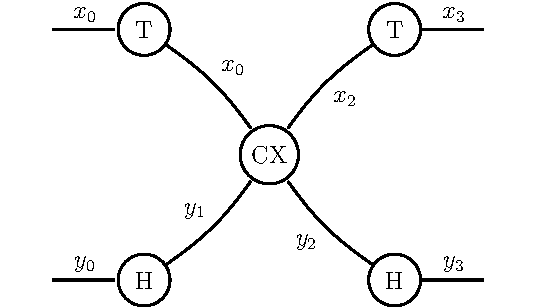
\includegraphics[width=.6\textwidth]{Img/tensor_example.pdf}
    \caption{用张量表示图\ref{fig:example_cir_2}中量子线路}   
    \label{fig:example_cir_map}
\end{figure}
假如需要知道图\ref{fig:example_cir_2}中,输入态为\(\ket{00}\)时,线路输出态的状态。
可以利用张量表示,即式子\ref{eq-tensor}计算可能的输出态。当式子\ref{eq-tensor}取\(x_0 = 0, y_0 = 0, y_1 = 0\)时计算过程如下:
\begin{equation}
    \begin{aligned}
\phi_{x_0x_0y_0y_3}\left(0000\right)&=\sum_{b_1,b_2=0}^{1}T\left(00\right)H\left(0b_1\right)CX\left(00b_1b_2\right)T\left(00\right)H\left(b_20\right)\\ 
    &=\sum_{b_1,b_2=0}^{1}1\cdot H\left(0b_1\right)CX\left(00b_1b_2\right)\cdot 1\cdot H\left(b_20\right)\\
        &=H\left(00\right)CX\left(0000\right)H\left(00\right)+H\left(00\right)CX\left(0001\right)H\left(10\right)\\
        &+H\left(01\right)CX\left(0010\right)H\left(00\right)+H\left(01\right)CX\left(0011\right)H\left(10\right)\\
        &=\frac{1}{\sqrt{2}}\cdot 1 \cdot \frac{1}{\sqrt{2}}+\frac{1}{\sqrt{2}}\cdot 0 \cdot\frac{1}{\sqrt{2}}\\
        &+\frac{1}{\sqrt{2}}\cdot 0 \cdot \frac{1}{\sqrt{2}}+\frac{1}{\sqrt{2}}\cdot 1 \cdot\frac{1}{\sqrt{2}}\\
        &= 1
    \end{aligned}
    \label{eq-ex_cal_1}
\end{equation}
类似地,当式子\ref{eq-tensor}取\(x_0 = 0, y_0 = 0, y_1 = 1\)时,结算结果为:
\begin{equation}
    \begin{aligned}
\phi_{x_0x_0y_0y_3}\left(0001\right)&=0
    \end{aligned}
\end{equation}
因此对图\ref{fig:example_cir_2}中的量子线路,输入态为\(\ket{00}\)时,线路输出态一定是\(\ket{00}\)。
\end{example}
\subsection{张量决策图}
张量决策图(Tensor Decision Diagrams,或TDD)是一种具有决策图和张量网络特征的数据结构\citep{Hong_2022}。它可用于表示张量和量子电路。与BDD(Boolean Decision Diagrams)类似,TDD是一种建立在索引顺序$I=\{x_1,\ldots,x_n\}$上的决策树模型。具体定义定义\ref{df-tdd}所示。
\begin{definition}
    \label{df-tdd}
    TDD是一个建立在索引顺序$I=\{x_1,\ldots,x_n\}$上的有根节点,带权重的有向无环图,其中包括:
    \begin{align}
        \mathcal{F}=\left(V,E,index,value,low,high,w\right)
    \end{align}
    其中:
    \begin{enumerate}
        \item $V$是一个有限节点集,被划分为非终端节点$V_n$和终端节点$V_T$。用$r_{\mathcal{F}}$表示$\mathcal{F}$的唯一根节点。
        \item $E=\left\{\left(v,low\left(v\right)\right),\left(v,high\left(v\right)\right):v\in V_N\right\}$是树中所有边集合,其中$\left(v,low\left(v\right)\right)$和$\left(v,high\left(v\right)\right)$分别称为v的低边和高边,分别指向该节点索引的负切片和正切片。根结点$r_{\mathcal{F}}$具有唯一的入射边$e_{\mathcal{F}}$,该入射边没有源结点。
        \item $index:V_r\rightarrow I$将每个非终端节点分配给I中的索引。
        \item $value:V_T\rightarrow\mathbb{C}$将每个终端节点赋予一个复数值。
        \item $low$和$high$都是$V_N\rightarrow V$中的映射,它们分别为每个非终端节点指定其低边和高边后继。
        \item $w:E\rightarrow\mathbb{C}$将每条边赋予一个复数权重。特别地,$w\left(e_r\right)$称为$\mathcal{F}$的权重,并记作$w_{\mathcal{F}}$。
    \end{enumerate} 
\end{definition}


对于TDD中的一个节点$v$,如果$v$是终端节点,则$\phi\left(v\right):= value (v)$是一个秩为$0$的张量,即常数,也可以称为一个平凡TDD。如果$v$是非终端节点,则根据定义,该节点表示的张量如式子\ref{eq-non-term}所示。
\begin{align}
    \label{eq-non-term}
    \phi(v):=w_{0} \cdot \overline{x_{v}} \cdot \phi(\operatorname{low}(v))+w_{1} \cdot x_{v} \cdot \phi(h i g h(v))
\end{align}
其中$x_v=index\left(v\right),\overline{x_{v}}=1-index\left(v\right)$。而整个TDD也可以表示为:
\begin{align}
    \phi\left(\mathcal{F}\right)=w_{\mathcal{F}}\cdot\phi\left(r_{\mathcal{F}}\right)
\end{align}

\begin{example}
    \label{ex-tdd}
    例子\ref{ex-tensor}给出了一个量子线路到张量网络的例子。将该张量网络转化为TDD,可以得到图\ref{fig:tdd_ex}。其中索引顺序$I=\{x_0,y_0,y_3\}$。非终端节点$V_n$用圆表示,终端节点$V_T$用方形表示。每个节点的低边用虚线表示,高边用实线表示。该示例中各边的权重均为1,即$w:E\rightarrow 1$。根节点的索引$index(r_{\mathcal{F}})=x_0$,即根节点\(r_{\mathcal{F}}\)是索引为\(x_0\)的节点。决策树的权重$w_{\mathcal{F}}=1$。

\begin{figure}[!htbp]
    \centering
    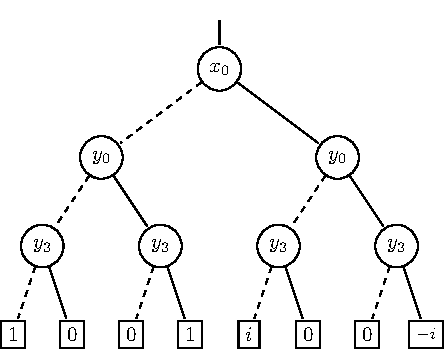
\includegraphics[width=.6\textwidth]{Img/tree_tdd.pdf}
    \caption{索引顺序$I=\{x_0,y_0,y_3\}$时图\ref{fig:example_cir_map}中的张量网络对应的TDD}   
    \label{fig:tdd_ex}
\end{figure}
当需要得到该TDD对应的张量网络中一个索引序列对应的值时,只需要知道图\ref{fig:tdd_ex}中索引对应的边所和连接的最后终端节点的值。将边的权重与最后的终端节点的值乘积起来,就可以知道该索引取值对应的值。
比如式子\ref{eq-ex_cal_1}计算的\(x_0 = 0, y_0 = 0, y_1 = 0\)所对应的边是图\ref{fig:tdd_ex}中最左边的虚线,而对应的终端节点是最左边的终端节点,因此该张量网络中:
\begin{equation}
    \begin{aligned}
\phi_{x_0x_0y_0y_3}\left(0000\right)
    = 1\cdot 1\cdot 1\cdot 1 = 1
    \end{aligned}
\end{equation}
类似地,\(x_0 = 0, y_0 = 0, y_1 = 1\)对应的终端节点是左边起,第二个的终端节点,因此:
\begin{equation}
    \begin{aligned}
\phi_{x_0x_0y_0y_3}\left(0001\right)
= 1\cdot 1\cdot 1\cdot 0 = 0
    \end{aligned}
\end{equation}
\end{example}
\subsection{TDD的规范与化简}
从例子\ref{ex-tdd}中得到TDD,可以看到由于图中边的权重信息使用较少,因此根据定义得到的TDD在结构上显然比较冗余,可以进行进一步化简。具体过程是先进行规范化(normalized),让后进行化简(reduced)\citep{Hong_2022}。
其中规范化的目的是使得TDD的终端节点只包含0和1,同时将终端节点的张量值沿路径逐步上移。具体规范步骤如下:
\begin{enumerate}
    \item 如果$v$是一个非零值$value\left(v\right)\neq 1$的终端节点,则将其值设置为1,并将每个入边的权重w更改为$value\left(v\right)\cdot w$。\label{norm1}
    \item 假设v是一个非终端节点,且$\phi\left(v\right)\neq 0$。首先规范化$\phi\left.\left(low(v\right)\right)$和$\phi\left.\left(high(v\right)\right)$。完成$\phi\left.\left(low(v\right)\right)$和$\phi\left.\left(high(v\right)\right)$的规范化后。如果$\phi\left.\left(low(v\right)\right)\neq 0$,并且此时$\phi\left.\left(high(v\right)\right)=0$或$\left|w_0\right|\geq\left|w_1\right|$,则将$w$设置为$w_0$。否则,将$w$设置为$w_1$。然后更新$w_0≔w_0/w,w_1≔w_1/w$。此时完成$v$的规范化。\label{norm2}
\end{enumerate}



在完成规范化后,此时的TDD终端节点只包含0和1。可以进一步简化TDD,使得TDD只包含一个终端节点1,同时尽量使用重复出现的张量。具体简化步骤如下:
\begin{enumerate}
    \item 	合并所有值为1的终端节点。删除所有终端$0$节点,并将它们的入边重定向到唯一的终端节点,并将它们的权重重置为$0$。\label{sympl1}
	\item 将所有权重为$0$的边重定向到终端节点。如果根节点的入边权重为$0$,则终端节点成为新的根,该TDD为空。删除所有从根节点不可达的节点,以及涉及它们的所有边。\label{sympl2}
	\item 如果一个节点v的低边和高边后继相同,并且其低边和高边具有相同的权重w,则删除该节点。如果入边权重$w=0$,则将其传入边重定向到终端节点。否则,将其传入边重定向到其后继节点。\label{sympl3}
	\item 合并两个具有相同索引、相同$0$和$1$后继以及对应边上相同权重的节点。\label{sympl4}
\end{enumerate}

\begin{example}
    对于例子\ref{ex-tdd}中的TDD。具体规范化过程为:应用第\ref{norm1}步于$i$和$-i$两个终端节点得到图表 \ref{fig:tdd-norma};然后,应用第\ref{norm2}步于右侧两个$y_3$节点,得到图表 \ref{fig:tdd-normb};最后,应用第二条规则于于右侧$y_0$节点。最后可以获得图表 \ref{fig:tdd-normc}。
比如对于图\ref{fig:tdd-normc}中规范TDD。具体化简过程为:首先重复第\ref{sympl1} 步,合并所有终端节点,得到图\ref{fig:tdd-redu1};由于没有符合第\ref{sympl2}和第\ref{sympl3}步的节点,因此直接进行第\ref{sympl4}步应用重复第四条规则合并第一个和第三个$y_3$节点,以及第二个和第四个$y_3$节点。最终可以得到\ref{fig:tdd-redu2}所示的简化TDD。
\begin{figure}[!htbp]
    \centering
    \begin{subfigure}[b]{0.4\textwidth}
        \centering
        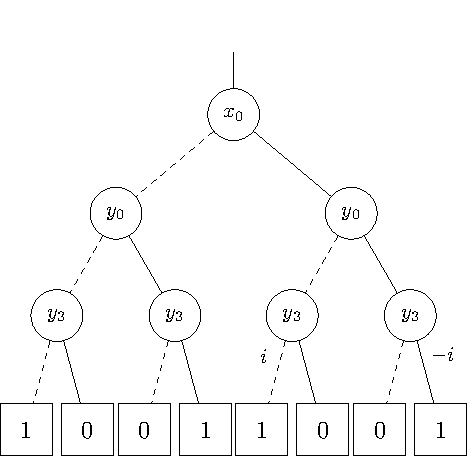
\includegraphics[height=5cm]{Img/tree_norm1.pdf}
        \caption{对图\ref{fig:tdd_ex}的终端节点规范化}
        \label{fig:tdd-norma}
    \end{subfigure}
    \begin{subfigure}[b]{0.4\textwidth}
        \centering
        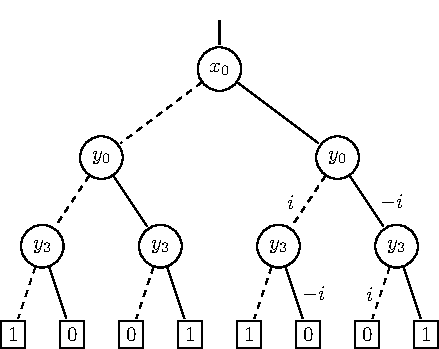
\includegraphics[height=5cm]{Img/tree_norm2.pdf}
        \caption{对图\ref{fig:tdd-norma}的$y_3$节点规范化}
        \label{fig:tdd-normb}
    \end{subfigure}
    \\
    \begin{subfigure}[b]{0.8\textwidth}
        \centering
        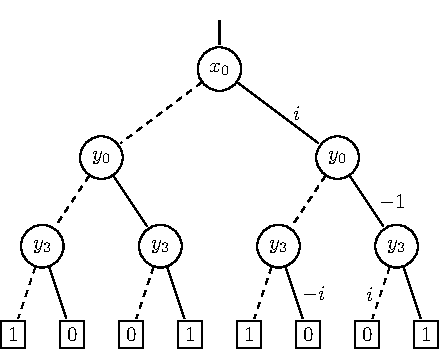
\includegraphics[width=.8\textwidth]{Img/tree_norm3.pdf}
        \caption{对图\ref{fig:tdd_ex}的规范化结果}
        \label{fig:tdd-normc}
    \end{subfigure}
    \caption{对图\ref{fig:tdd_ex}的规范化过程}
    \label{fig:tdd-norm}
\end{figure}
\begin{figure}[!htbp]
    \centering
    \begin{subfigure}[b]{0.4\textwidth}
        \centering
        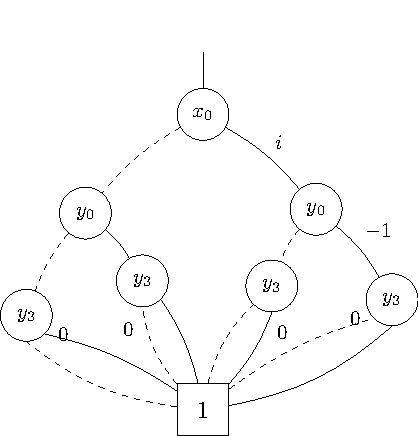
\includegraphics[height = 6cm]{Img/tree_redu1.pdf}
        \caption{对\ref{fig:tdd-normc}中规范TDD的终端节点化简}
        \label{fig:tdd-redu1}
    \end{subfigure}
    \begin{subfigure}[b]{0.4\textwidth}
        \centering
        \includegraphics[height = 6cm]{Img/tree_redu2.pdf}
        \caption{对图\ref{fig:tdd-normc}中规范TDD的简化结果}
        \label{fig:tdd-redu2}
    \end{subfigure}
    \caption{对图\ref{fig:tdd-norm}的化简过程}
    \label{fig:tdd-redu}
\end{figure}
\end{example}

为了阅读简洁,下文中无特殊说明的TDD均指化简后的TDD,即reduced tensor decision diagrams。结合以上步骤,算法\ref{alg-tdd}简单展示了如何将给定的张量\(\phi\)转换为对应的TDD表示。
\begin{algorithm}
    \caption{生成张量\(\phi\)的TDD表示TDD(\(\phi\))}
    \label{alg-tdd}
    \begin{algorithmic}[1]
    \Require 一个张量\(\phi\) 和对应的索引顺序\(I\)
    \Ensure \(\phi\)的TDD表示TDD(\(\phi\))
    \If{\(\phi = c\),即输入张量是一个标量}
        \State \Return 带权重$c$的平凡TDD
    \EndIf
    \State \(x \gets\) \(\phi\)在索引顺序\(I\)中最小的索引
    \State \(tdd \gets\) 一个空的TDD
    \State \(tdd.root \gets\) 一个索引为\(x\)的新节点\(v\) 
    \State \(v.low \gets\) 递归调用本算法,得到\(\phi|_{x=0}\)对应的TDD表示TDD(\(\phi|_{x=0}\))
    \State \(v.high \gets\) 递归调用本算法,得到\(\phi|_{x=1}\)对应的TDD表示TDD(\(\phi|_{x=1}\))
    \State \(tdd.weight \gets 1\)
    \State \Return \(tdd\)化简后的TDD表示
    \end{algorithmic}
\end{algorithm}


\subsection{TDD之间的运算}
TDD是基于张量网络的数据结构,因此张量之间的基础操作也会在TDD有所对应。
用张量网络表示量子电路时,将大量应用张量加法和张量收缩(contraction)。因此本小节主要介绍不同TDD之间的加法和收缩。
\subsubsection*{TDD之间的加法}
张量网络中,两个张量的加法是将两个具有相同维度的张量在对应元素上进行加和的操作,结果是一个新的张量。这种操作在处理张量网络时用于合并具有相同结构但不同数据的张量。在TDD中,加法操作通过递归地合并两个TDD的节点来实现,对应于在张量网络中将两个张量相加,从而形成一个表示两者之和的新的张量网络。具体算法如算法\ref{alg-add}。
\begin{algorithm}
\caption{对具有相同索引的两个TDD表示\(\mathcal{F}, \mathcal{G}\)进行加法运算}
\label{alg-add}
\begin{algorithmic}[1]
\Require 两个简化后的TDD表示\(\mathcal{F}\)和\(\mathcal{G}\),以及对应的索引顺序\(I\)
\Ensure \(\mathcal{F} + \mathcal{G}\)的TDD表示
\If{\(r_{\mathcal{F}}\) 等于\(r_{\mathcal{G}}\),即两个TDD的结构完全一致}
    \State \(tdd \gets \mathcal{F}\)
    \State \(tdd.weight \gets w_{\mathcal{F}} + w_{\mathcal{G}}\)
    \State \Return \(tdd\)
\EndIf
\State \(x \gets\) 索引顺序\(I\)下\(\mathcal{F}\)和\(\mathcal{G}\)最小的相同索引\(r_{\mathcal{F}}\) 和 \(r_{\mathcal{G}}\)
\State \(tdd \gets\) 一个空的TDD
\State \(tdd.root \gets\) 一个索引为\(x\)的新节点\(v\)
\State \(v.low \gets\) 递归调用本算法,计算\(\mathcal{F}_{x=0} + \mathcal{G}_{x=0}\)对应的TDD表示
\State \(v.high \gets\) 递归调用本算法,计算\(\mathcal{F}_{x=1} + \mathcal{G}_{x=1}\)对应的TDD表示
\State \(tdd.weight \gets 1\)
\State \Return \(tdd\)化简后的TDD表示
\end{algorithmic}
\end{algorithm}

\subsubsection*{TDD之间的收缩}
张量收缩是张量网络中最核心的操作之一,它指的是沿着一个或多个共享维度对张量进行求和的过程,从而减少张量的总维数。这个操作在量子物理和量子计算的模拟中特别重要,因为它能够模拟多个量子态或量子门的相互作用。在TDD中,收缩操作通过在特定变量集上合并节点来实现,模拟了在张量网络中按照给定维度进行张量收缩的过程。具体算法如算法\ref{alg-cont}所示。
\begin{algorithm}
\caption{对两个TDD表示\(\mathcal{F}, \mathcal{G}\)收缩所有在\(\text{var}\)集合中的索引}、
\label{alg-cont}
\begin{algorithmic}[1]
\Require 两个TDD表示\(\mathcal{F}\)和\(\mathcal{G}\),以及对应的索引顺序\(I\)和需要收缩的索引集合\text{var}
\Ensure 通过在 $\text{var}$ 上合并 \(\mathcal{F}\) 和 \(\mathcal{G}\) 获得的简化的TDD
\If{\(\mathcal{F}\)和\(\mathcal{G}\)都是平凡TDD}
    \State \(tdd \gets \mathcal{F}\)
    \State \(tdd.weight \gets w_{\mathcal{F}} \cdot w_{\mathcal{G}} \cdot 2^{\text{len}(\text{var})}\)
    \State \Return \(tdd\)
\EndIf
\State \(x \gets\) 索引顺序\(I\)下\(\mathcal{F}\)和\(\mathcal{G}\)最小的相同索引\(r_{\mathcal{F}}\) and \(r_{\mathcal{G}}\)
\State \(L \gets \) 递归调用本算法,得到\(\mathcal{F}_{x=0}, \mathcal{G}_{x=0}\)在收缩索引集合\(\text{var}\setminus\{x\}\)的TDD表示
\State \(R \gets \) 递归调用本算法,得到\(\mathcal{F}_{x=1}, \mathcal{G}_{x=1}\)在收缩索引集合\(\text{var}\setminus\{x\}\)的TDD表示
\If{\(x \in \text{var}\)}
    \State \(tdd \gets\) 调用算法\ref{alg-add},得到\(L, R\)的和
    \State \Return $tdd$
\Else
    \State \(tdd \gets\) 一个空的TDD
    \State \(tdd.root \gets\) 一个索引为\(x\)的新节点\(v\)
    \State \(v.low \gets L\)
    \State \(v.high \gets R\)
    \State \(tdd.weight \gets 1\)
    \State \Return \(tdd\)化简后的TDD表示
\EndIf
\end{algorithmic}
\end{algorithm}

\section{对比类似表示}
\label{sec-compare}
TDD是一种相对较新的数据结构,用于表示和操作张量网络。张量网络提供了量子线路更紧凑的表现形式。本小节中将对比TDD,直接使用张量网络TN,以及QMDD\citep{1623982}三种表示的效率。

QMDD(Quantum Multiple-Valued Decision Diagrams),即量子多值决策图提供了一种紧凑而系统的方法来描述量子过程。目前QMDD已有效地用于量子电路的合成\citep{niemann2020advanced}和和验证任务
\citep{burgholzer2020verifying,burgholzer2020advanced}。
图\ref{fig:qmdd-basic}展示了一个矩阵到最终QMDD的一个过程。
\begin{figure}[htbp]
    \centering
    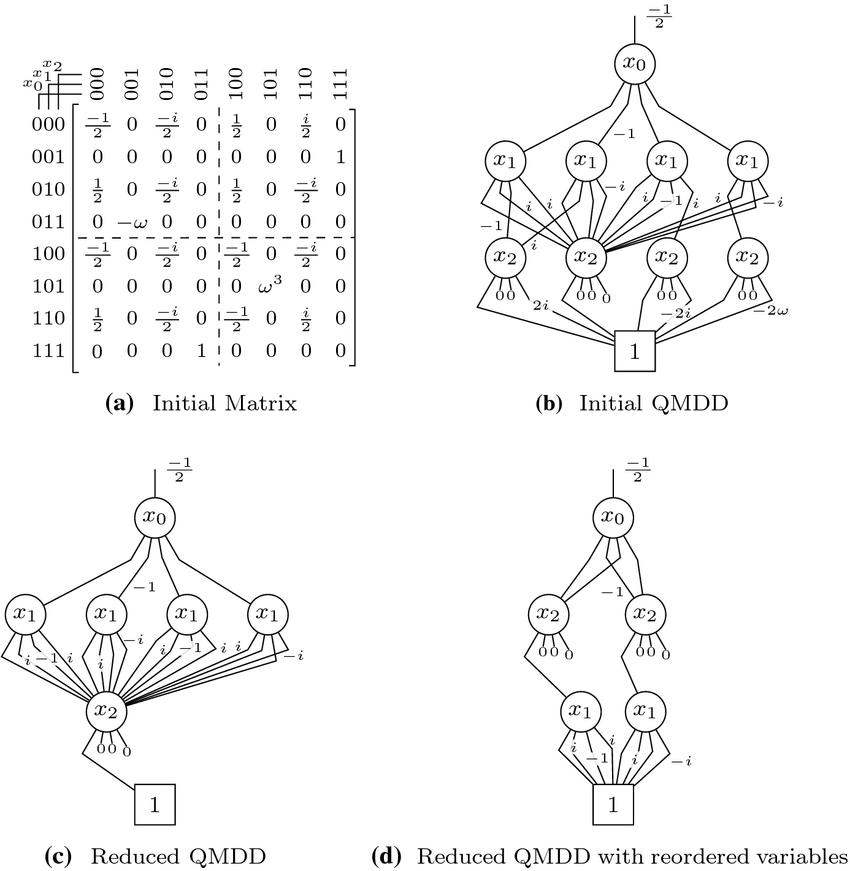
\includegraphics[height=10cm]{Img/QMDD-intro}
    \caption{一个QMDD的示例}
    \label{fig:qmdd-basic}
\end{figure}

可以看到QMDD和TDD的相似点有:
\begin{enumerate}
    \item 二者都存在唯一的终端顶点,值为1。该终端顶点没有出边。
    \item 二者都有唯一一个顶点作为起始顶点,它有一个单独的入边,该入边本身没有源顶点。
    \item 二者中的每条边(包括指向起始顶点的边)都有一个关联的复数值权重。
    \item 二者中的索引都按一定顺序排列,并且都满足以下两条规则:
    \begin{enumerate}[label=\roman*)]
        \item 每个索引在从起始顶点到终端顶点的每条路径上最多出现一次。
        \item 来自索引排序低的非终端顶点的边指向索引排序高的非终端顶点或终端顶点。
    \end{enumerate}
    \item 二者都尽量复用节点,即没有两个标记索引相同的非终端顶点有相同的出边集(即连接节点和边权重都一致)。
\end{enumerate}

QMDD和TDD主要不同的在于QMDD结构中,每个非终端节点连接有四个后继节点。
而在TDD结构中,每一个非终端节点分别连接着两个后继节点。从原理上讲,如果采用相同的排序规则,量子电路的TDD表达方式的节点数大约是其QMDD表达方式节点数的两倍。此时TDD表达方式所需的内存空间大约与QMDD表达方式所需的内存空间持平。这是因为它们都拥有相同数目的加权边并记录了相同数量的权值(即复数)。
因此TDD的表示形式和QMDD紧凑程度相近。
然而TDD由于可以轻松与张量网络中的一些优化技术结合以进一步提高其表现。

比如在TDD原文中\citep{Hong_2022},就介绍了两种通过分区进行优化的方案,TDD part I和 TDD part II。TDD part I 分区方案侧重于如何将量子门分组到不同的分区中,以优化TDD的表示效率和计算性能。而TDD part II 分区方案中,重点是如何根据比特之间的相互作用和关联性将它们分配到不同的分区中。

TDD part I分区方案中通过中间水平方向将电路分割为上下两等部分,确保每部分包含的比特数目大致相等。接着,电路会被垂直方向切割,以此确保在任一分区中,由水平切割线分隔的CX门的数量不会超过预设的参数$k$。
\begin{example}
    以图\ref{fig:tdd-part-I}中的量子线路为例。
由于线路中有四个比特,因此水品分割线将线路分割为上下各两个比特。此时虚线框的两个CX被水平分割线分割。因此当取\(k=1\)时,可以将线路划分为图\ref{fig:tdd-part-I}中的\(A1\),\(A2\),\(B1\),\(B2\)四部分。
\begin{figure}[!htbp]
    \centering
    \includegraphics[height=4.5cm]{Img/tdd-part-I.pdf}
    \caption{TDD part I分区方案的例子,其中预设参数\(k=1\)}
    \label{fig:tdd-part-I}
\end{figure}
\end{example}

TDD part II分区方案是基于\citep{huang2020classical}中用于传统模拟的策略的扩展。在方案中首先与第一种方案类似,从电路中部进行水平划分。当预定义的参数$k1$个CX门因为水平分割而分开时,会设立一个新的小区块。这个小区块包含电路的一小部分,内含数个因水平切割而分隔的CX门,即这些门在此区块内不与区块外的比特发生任何交互。每当这个小区块涉及到预定义的参数$k2$比特时,就进行一次新的垂直分割。
\begin{example}
    同样以图\ref{fig:tdd-part-I}中的量子线路为例。水平分割线分割后,此时虚线框的两个CX被水平分割线分割。因此当取\(k1=1\)时,将右边虚线框的CX设立在小区块\(C\)中。当取\(k2=2\)时,小区块\(C\)的比特数限制到2。因此可以将线路划分为图\ref{fig:tdd-part-II}中的\(A1\),\(A2\),\(C1\),\(B1\),\(B2\)四部分。
\begin{figure}[!htbp]
    \centering
    \includegraphics[height=4.5cm]{Img/tdd-part-II.pdf}
    \caption{TDD part II分区方案的例子,其中预设参数\(k1=1,k2=2\)}
    \label{fig:tdd-part-II}
\end{figure}
\end{example}
% 图\ref{fig:zx-basic}展示了ZX-calculus中量子计算基本门的形式。图\ref{fig:zx-rule}展示了ZX-calculus的基本化简规则。将一个量子线路中的比特门表示为Z-calculus后化简,从而进行验证。

% \begin{figure}[!htbp]
%     \centering
%     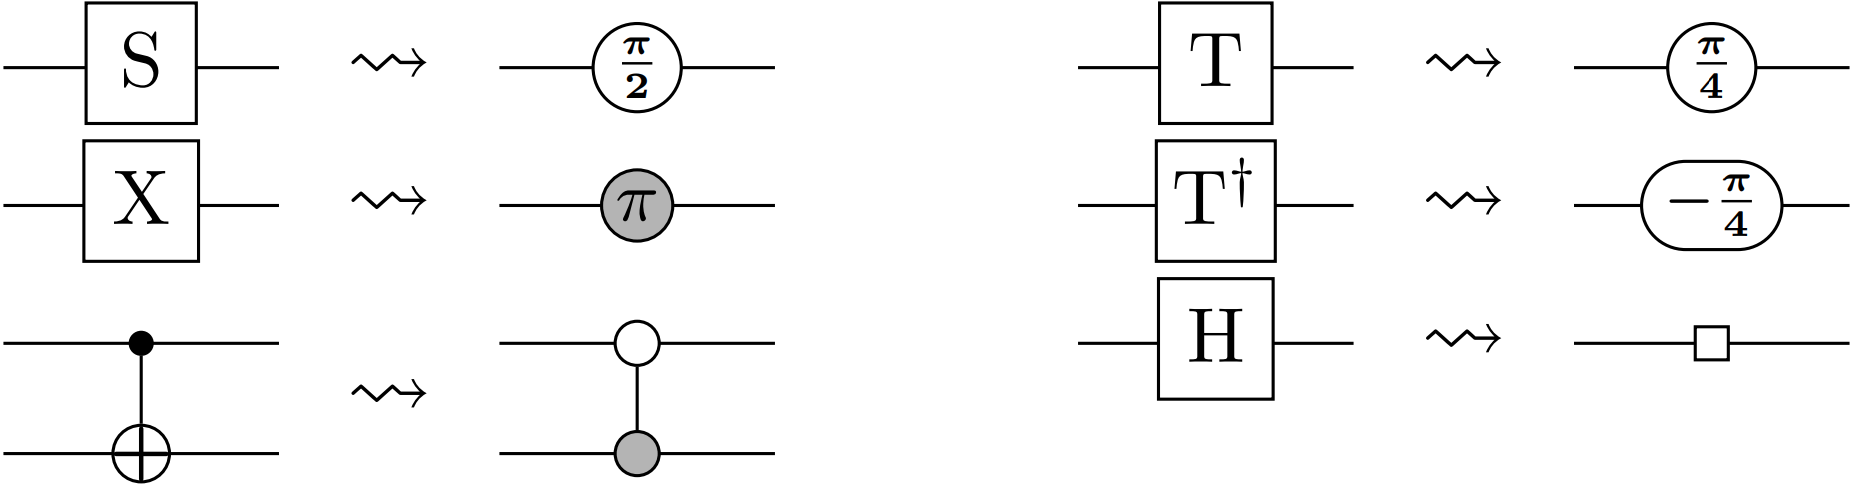
\includegraphics[height=4cm]{Img/zx-basic.pdf}
%     \caption{量子计算基本门在ZX-calculus的表示}
%     \label{fig:zx-basic}
% \end{figure}
% \begin{figure}[!htbp]
%     \centering
%     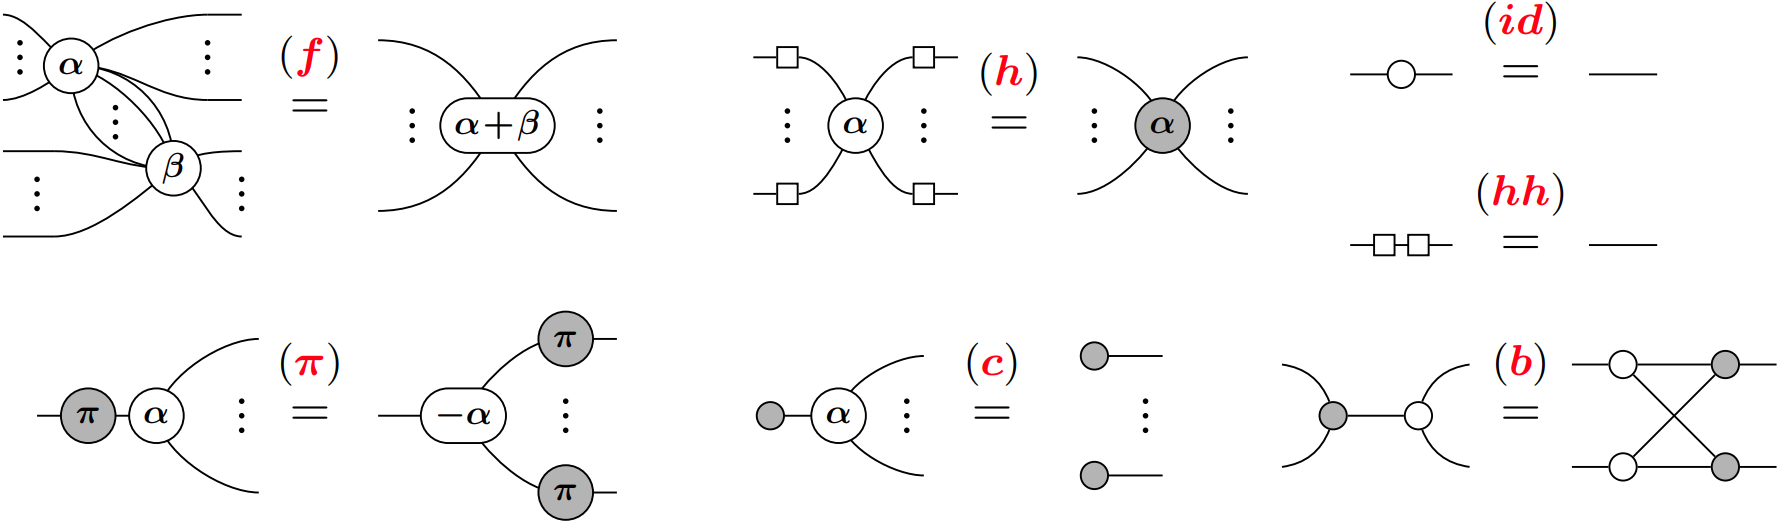
\includegraphics[height=4cm]{Img/zx-rule.pdf}
%     \caption{ZX-calculus的基本化简规则}
%     \label{fig:zx-rule}
% \end{figure}
 
% 目前ZX-calculus发展还比较早期。
% //TODO: add TN 
图\ref{fig:tdd-compare}展示了目前各种比较成熟的表示方法下模拟量子电路的时间对比。其中TDD No Part指的是不对电路进行拆分优化的方法。TDD part I 和TDD part II都是是前文中提到的优化方案。
QMDD指的是QuantumMultiple-valued Decision Diagrams。
TN是指google的tensor network。
从图\ref{fig:tdd-compare}可以看到,两种TDD的优化方案都是时间消耗最少的。不使用拆分优化的TDD No Part与QMDD时间接近。而当比特数少于10时,TN的时间少于TDD No Part,但随着比特数增加,TN的用时快速超过TDD No Part。
因此TDD相比其他表示方式有一定优势。这是本次研究选择TDD作为主要技术的重要原因。

\begin{figure}[!htbp]
    \centering
    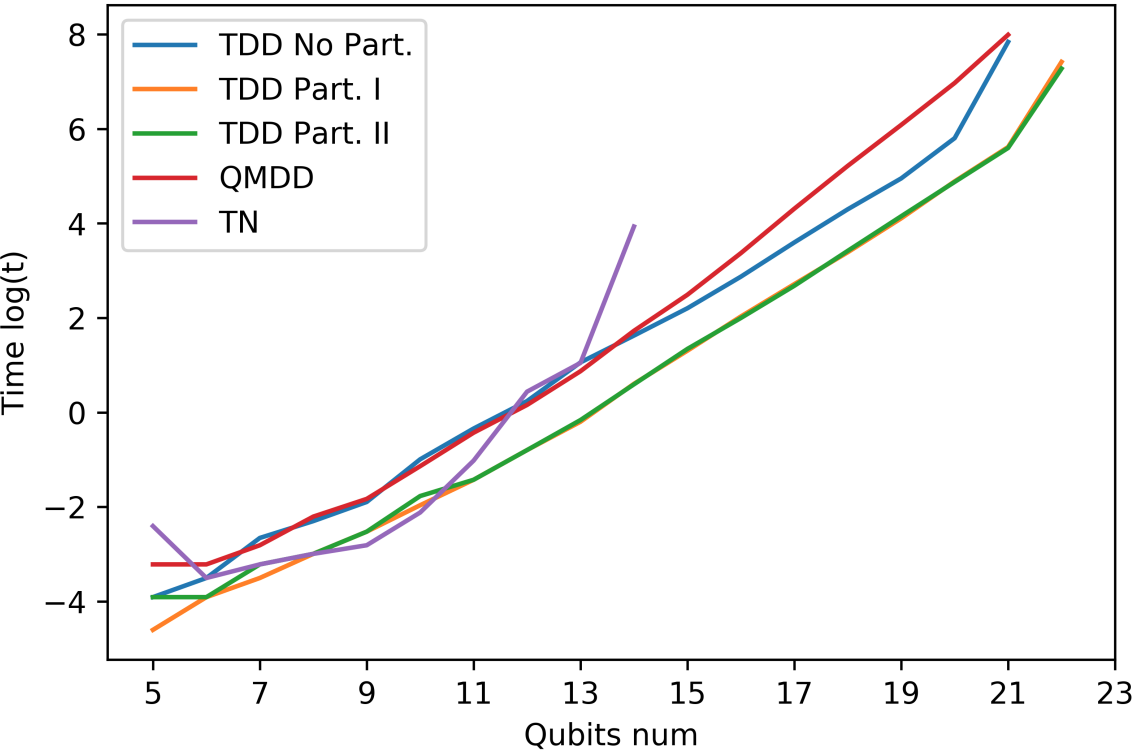
\includegraphics[height=8cm]{Img/tdd-compare.pdf}
    \caption{对QFT电路,TDD与TN,QMDD表示的比较\citep{Hong_2022}}
    \label{fig:tdd-compare}
\end{figure}

目前,TDD研究集中在开发更有效的算法来使用TDD操作和收缩张量网络。这包括开发新技术来分割张量网络,优化TDD结构,从而进一步提高基于TDD的可达性分析和模型检测算法的效率。这也是实现基于TDD的量子模型检测的主要方法。

\section{在模型检验中应用TDD}
借助新的数据结构TDD,可以更方便的表示量子状态以及量子线路,并计算最终的结果。同时TDD特别适用于实现可达性分析和模型检查算法。这是因为基于BDD的模型检查算法中使用的许多优化技术可以推广到收缩量子电路张量网络上\citep{Chaki_2018}。这些为应用TDD解决量子模型检测问题提供了可能的方案。

在\ref{sec-transition}节中介绍了跃迁系统,其中式子\ref{eq:image}给出了量子跃迁系统的简单定义。这里简单回顾以一下。对于一个希尔伯特空间$\mathcal{H}$ 。基于 $\mathcal{H}$ 的量子转移系统 $\mathcal{M}$ 可以表述为四元组 $(\mathcal{H}, S_0, \Sigma, \mathcal{T})$,这里 $S_0$ 作为 $\mathcal{H}$ 的一个封闭子空间,被定义为初始空间。$\Sigma=\{\sigma_1,\ldots,\sigma_m\}$ 是一系列符号集合,$\mathcal{T}=\mathcal{T}_\sigma, {\sigma \in \Sigma}$ 则代表对 $\mathcal{H}$ 执行的一组量子操作。


\begin{example}
    一个单量子比特的系统可能遭受两种潜在的噪声影响:比特位翻转和相位翻转。如果不能准确判断会发生哪一种噪声,这样的系统可以被表达为一个量子转移系统 $\mathcal{M}=\big(\mathcal{H}_2,S_0,\{1,2\},{\mathcal{T}_1,\mathcal{T}_2} \big)$,这里 $S_0$ 代表 $\mathcal{H}$ 中的一个子空间,$\mathcal{T}_1=\{\sqrt{p}I, \sqrt{1-p}X\}$ 和 $\mathcal{T}_2=\{\sqrt{p}I, \sqrt{1-p\}Z}$。 $I,X,Z$ 分别代表恒等矩阵、Pauli $X$ 矩阵和Pauli $Z$ 矩阵。
\end{example}
\begin{example}
    \label{ex-image-grover}
    量子线路也可以表达为一个量子迁移系统。图\ref{fig:grover}展示了实现两量子比特 Grover 迭代的电路 \citep{Grover_1996},这是 Grover 算法的一个基本过程,用于找到布尔函数 $f(x)=1$ 的解。该类算法需要验证的属性是能否始终进入布尔函数解所在的子空间。
    对于该电路,第一个 CCX 门表示搜索用的oracle,实现了$ O\ket{x}\ket{y}=\ket{x}\ket{f(x)\oplus y}$,其中 $f(x)=x_1 \wedge x_2$。因此,该电路oracle的解是\(00\) 。其他门实现了一个补$2\ket{\psi}\bra{\psi}-I$,其中$\ket{\psi}=\frac{1}{\sqrt{2}^{n}}\sum_{i=0}^{2^n-1}\ket{i}$。给定输入状态 $\ket{++-}=\frac{1}{2}\sum_{i=0}^3\ket{i}\ket{-}$,电路首先将状态变为 $\frac{1}{2}\sum_{i=0}^2 \ket{i}\ket{-}-\frac{1}{2}\ket{11}\ket{-}$,然后变为 $\ket{11}\ket{-}$。对于状态空间 $S=span\{\ket{++-},\ket{11-}\}$。当目前系统状态 $\ket{\varphi} \in S$,下一步系统状态总会在 $S$ 中。

    因此该系统可以表示为量子迁移系统 $(\mathcal{H}_8, S, {1}, \mathcal{T})$ 进行建模,其中 $\mathcal{T}_1 = {(2\ket{\psi}\bra{\psi}-I) O}$,需要检查的属性是$\mathcal{T}_1(S)=S$。
    \begin{figure}[!htbp]
        \centering
        \includegraphics[height=4cm]{Img/cir_grover.pdf}
        \caption{Grover\_3的量子线路图}
        \label{fig:grover}
    \end{figure} 
\end{example}

\subsection*{子空间的表示}
在量子模型检测中,需要用到子空间的表示。一种表示子空间的办法是将子空间表示为一组基态。
给定子空间投影算子的矩阵形式,如果有一个非零的列向量,那么在该向量的方向上就可以找到一个基向量。然后,通过正交化过程,可以递归地找到原始子空间的一组正交基向量。
但是使用矩阵表示进行所有列的遍历会遇到很高的复杂度。而通过使用子空间投影算子的TDD表示,就可以可以容易地找到第一个非零列。
具体方法是寻找该TDD表示的最左侧非零路径。
通过这种图的方法避免了在计算过程中需要显式表示相应的向量,也减少了0复杂度​​。
综上所述,算法\ref{alg-basis_dec}给出了一个计算子空间的一组计算基的方法。在此算法基础上,可以给出根据当前系统状态计算下一步系统状态的算法\ref{alg-image}.
\begin{algorithm}
\caption{给出投影算子$P$的一组正交基}
\label{alg-basis_dec} 
\begin{algorithmic}[1]
    \Require 子空间$S$的TDD形式投影算子$P=P_S$ 
    \Ensure $P$的一组正交基分解$B$
    \State $B\gets \{\}$
    \If{\(P\) 是空的} 
        \Return \(B\)
    \Else
        \State \(\ket{i} \gets\) TDD表示\(P\)中最左侧非零路径所表示的列号\(i\)
        \State \(\ket{u_i}\gets\) 由在TDD表示\(P\) 中具有列号 \(\ket{i}\) 的路径表示的状态
        \State \(\ket{v_i} \gets \frac{\ket{u_i}}{\|\ket{u_i}\|}\)
        \State \(P \gets P - \ket{v_i}\bra{v_i}\)
        \State \(B' \gets \) 递归调用本算法,得到新的$P$的计算基分解
        \State \(B \gets B \cup \{\ket{v_i}\} \cup B'\)
    \EndIf
    \State \Return \(B\)
\end{algorithmic}
\end{algorithm}

\begin{example}
    \label{ex-image-sub}
    例子\ref{ex-image-grover}将Grover算法的电路建模为量子迁移系统。其中用到了子空间$S=span\{\ket{++-},\ket{11-}\}$。相应投影算子 $P$ 的矩阵和 TDD 表示如图 \ref{fig:P} 所示。
    根据该TDD表示求解原子空间的基的过程如下:
    \begin{enumerate}
        \item 应用图算法,得到最左侧路径对应于 $(x_1,x_2,x_3,y_1,y_2,y_3)=(0,0,0,0,0,0)$,这意味着投影算子的第一列非零。
        \item 遍历所有 $(x_0,x_1,x_2)=(0,0,0)$ 的路径,得到向量 $\ket{v_1}=\frac{1}{6}[1,-1,1,-1,1,-1,0,0]$。
        \item $\ket{v_1}$标准化为 $\ket{v_1}=\frac{1}{\sqrt{3}}(\ket{00}+\ket{01}+\ket{10})\ket{-}$。
        \item 设 $P'=P-\ket{v_1}\bra{v_1}$。那么 $P'$ 等于 $\ket{11-}\bra{11-}$。
        \item 对 $P'$ 重复上述的过程,获得 另一组基$\ket{v_2}=\ket{11}\ket{-}$,此时TDD为空。因此 ${\ket{v_1},\ket{v_2}}$ 是子空间 $S$ 的一个基。
    \end{enumerate}
\end{example}
\subsection*{子空间的并}
子空间的并也是模型检测中重要的一步。设 $S=S_1\vee S_2$ 为两个子空间 $S_1,S_2$ 的并集。假设 $B_1=\{\ket{\psi_{11}},\cdots,\ket{\psi_{1k}}\}$ 和 $B_2=\{\ket{\psi_{21}},\cdots,\ket{\psi_{2l}}\}$ 分别是 $S_1$ 和 $S_2$ 的一组正交基。子空间$S$的一组正交基$B$可以通过格拉姆-施密特正交化方法(Gram–Schmidt process)计算而来,具体方法如下。
\begin{enumerate}
    \item 令 $B=B_1$,并定义 $P=\sum_{j=1}^{k}{\ket{\psi_{1j}}\bra{\psi_{1j}}}$。
    \item 遍历$B_2$ 中的基向量。假设当前向量为 $\ket{\psi_{2j}}$。计算 $\ket{u_j}=\ket{\psi_{2j}}-P\ket{\psi_{2j}}$ 并将其标准化为 $\ket{v_j}=\frac{\ket{u_j}}{|\ket{u_j}|}$。
    \item 如果 $\ket{v_j}$ 为 0,则考虑下一个向量;否则,此时它与 $P$ 正交,将其添加到 $B$ 中。同时,还将 $P$ 更新为 $P+\ket{v_j}\bra{v_j}$。
    \item 重复上述过程直到遍历完 $B_2$ 中的所有元素。此时$B$ 将成为 $S$ 的一个基,$P$ 将成为到 $S$ 的投影算子。
\end{enumerate}

这个过程展示了如何从一组生成向量开始,通过计算和正交化过程,构建出一个复合空间的正交归一化基。在量子计算和量子信息中,这种方法特别有用,因为它允许准确地描述和操控量子态的子空间。

\begin{example}
    例子\ref{ex-image-grover}中对Grover 3电路建模,例子\ref{ex-image-sub}对涉及的子空间进行了分解。考虑分解的逆过程,设 $P_1,P_2$ 为两个一维子空间 $S_1,S_2$ 的投影算子,分别由 $B_1=\{\ket{++-}\}$ 和 $B_2=\{\ket{11-}\}$ 生成。显然,$P_1=\ket{++-}\bra{++-}$。将 $B_1$ 完善为 $S=S_1\vee S_2$ 的一个基。计算得到$\ket{u}=\ket{11-}-P_1\ket{11-}=\ket{11-}-\frac{1}{4}\ket{++-}=[-\frac{1}{4},\frac{1}{4},-\frac{1}{4},\frac{1}{4},-\frac{1}{4},\frac{1}{4},\frac{3}{4},-\frac{3}{4}]^T$,可以被标准化为 $\ket{v}=-\frac{1}{2\sqrt{3}}(\ket{00}+\ket{01}+\ket{10}-3\ket{11})\ket{-}$。那么 $B=\{\ket{++-},\ket{v}\}$ 是一个正交归一化基,且 $P=P_1+\ket{v}\bra{v}$ 是相应的投影算子。
\end{example}
\subsection*{计算一步迁移}
结合子空间的分解算法,可以给出对于量子系统的一步映射算法,具体如\ref{alg-image}所示。
\begin{algorithm}
\caption{基于迁移系统的一步映射算法}
\label{alg-image}
\begin{algorithmic}[1] % The optional argument [1] enables line numbering
\Require 一个量子迁移系统 $(\mathcal{H},S,\Sigma,\mathcal{T})$, 其中转移关系$\mathcal{T}=\{\mathcal{T}_\sigma\mid \sigma\in \Sigma\}$,  $\mathcal{T}_\sigma=\{E_{\sigma,j_\sigma}\}$
\Ensure 系统下一步状态$\mathcal{T}(S)$的投影算子$P$
\State $P \gets 0$ 
\State $B \gets $调用算法\ref{alg-basis_dec},得到$S$的计算基分解
\State $K \gets \cup_{\sigma,j_\sigma}\{E_{\sigma,j_\sigma}\}$
\For{$\ket{\psi}$ \textbf{在} $B$, $E$ \textbf{在} $K$}
    \State $\ket{\phi} \gets $调用算法\ref{alg-cont},得到\(\ket{\psi}\)和\(E\) 合并所有相同索引的收缩
    \State $P=P \vee \text{span}\{\ket{\phi}\}$
\EndFor
\State \Return $P$ 
\end{algorithmic}
\end{algorithm}

在此基础上,可以计算该量子迁移系统$(\mathcal{H},S,\Sigma,\mathcal{T})$的可达空间。具体方法如下:
\begin{enumerate}
    \item 初始化可达空间为\(R = S\),并计算可达空间的投影算子\(P_{R}\)。
    \item 调用算法\ref{alg-image},计算系统$(\mathcal{H},S,\Sigma,\mathcal{T})$下一步状态\(S'=\mathcal{T}(S)\)。
    \item \label{it-be}调用算法\ref{alg-basis_dec},分解子空间得到\(S'\)的一组基\(B = \{\ket{\psi_{1}},\cdots,\ket{\psi_{n}}\}\)。同时初始化一个空的状态空间$S''$。
    \item 遍历\(B\)中的基,假设当前向量为\(\ket{\psi_{i}}\),计算得到\(\ket{u_i}=P\ket{\psi_{i}}\),并标准化为$\ket{v_j}=\frac{\ket{u_j}}{|\ket{u_j}|}$。
    \item \label{it-end}当$\ket{v_j}$为0时,考虑下一个向量;否则,此时$\ket{v_j}$与P正交,将该向量张开的空间并到子空间$S''$中,即$S''=S''\vee span\{\ket{v_j}\}$。同时更新可达空间$R=R\vee span\{\ket{v_j}\}$,即将 $P$ 更新为 $P+\ket{v_j}\bra{v_j}$。
    \item 遍历结束后,如果$S''$为空,说明该量子系统的可达空间已经收敛,即此时的$R$就是系统的可达空间。否则用$S''$作为量子系统的初态,计算迁移系统$(\mathcal{H},S'',\Sigma,\mathcal{T})$的下一步状态,并重复上述\ref{it-be}到\ref{it-end}的过程。
\end{enumerate}

\section{针对模型检测的改进}
本次研究的主要目的是借助TDD数据结构,构建能快速计算量子模型检测中可达问题的方案。本次研究的主要挑战在于尽可能减少程序的运行时间以及空间资源。为此,需要采用一系列方法来开发更有效的算法,以优化TDD操作和收缩张量网络。其中包括开发新技术来分割张量网络和优化TDD结构。下面简单介绍一下具体改进方法。

\subsection*{addition的拆分方案}
\label{addition}关于常用的量子线路划分方法,
第一种被称为addition\citep{chen2018classical}。将量子电路视为张量网络,首先将一个量子电路C转换成无向图G。G中的每个节点表示量子电路的一个索引,并且如果它们是相同门的输入或输出索引,则在G中连接两个节点。并且当满足以下两个条件之一时输入和输出索引不变:
\begin{itemize}
	\item 是对角线量子门的输入和输出索引;
	\item 是受控门的控制比特位的输入和输出索引。
\end{itemize}
在得到无向图后,就可以通过对连通度高索引进行张量切片,从而对量子电路进行划分。 
\begin{example}
    图\ref{fig:addition}展示了图\ref{fig:grover}中Grover\_3电路图的索引链接图。该图描述了量子电路的连通性,通过选择图中连通度最大的索引可以对电路进行分割。因此选择图中连通度较大的$x_1^1,x_1^3x_2^1$可以对电路进行较好的划分。
 
\begin{figure}[!htbp]
	\centering
	\includegraphics[height=6cm]{Img/cir_index_graph.pdf}
	\caption{Grover\_3的索引连接图}
	\label{fig:addition}
\end{figure} 
\end{example}

\subsection*{contraction的拆分方案}
另一种常用的电路划分方法成为contraction。该方法是\ref{sec-compare}小节中的TDD part I的延申。在这一方法中,将量子电路划分为若干个较小的部分,其收缩等于原始电路。应用两个预设整数参数$k1$和$k2$,将电路划分为若干小电路。其中每个小电路涉及最多$k1$个量子比特,并且与至多跨越不同部件的$k2$个多比特门相连。
\begin{example}
    图\ref{fig:contraction}展示了对Bit flip电路进行k1=3,k2=2的拆分结果。
\begin{figure}[!htbp]
	\centering
	\includegraphics[height=7cm]{Img/cir_contraction.pdf}
	\caption{对Bit flip电路进行contraction的拆分}
	\label{fig:contraction}
\end{figure} 
\end{example}


\subsection*{索引顺序的调整}
\label{contraction}在BDD中,索引的顺序很重要。因为索引顺序会直接影响BDD的大小。一个良好的变量顺序可以使得BDD比一个糟糕的变量顺序小得多。图\ref{fig:bdd-compare}的了两张图都表示了布尔函数$f (x1,...,x8)=x1x2+x3x4+x5x6+x7x8$,但图\ref{fig:bdd-good}的结构更简单。其中图\ref{fig:bdd-bad}的索引顺序为\{x1,x3,x5,x7,x2,x4,x6,x8\},图\ref{fig:bdd-good}的索引顺序为\{x1,x2,x3,x4,x5,x6,x7,x8\}。找到一个好的索引顺序是一个NP问题。在工程实现中,目前只能通过小规模电路上寻求规律,然后在更大规模电路中应用较优顺序。
% \textcolor{red}{目前也有一些研究借助xxx机器学习算法,寻找收缩的最佳序列\citep{zhang2024quantum}}
\begin{figure}[!htbp]
	\centering
	\begin{subfigure}[b]{.4\textwidth}
        \centering
        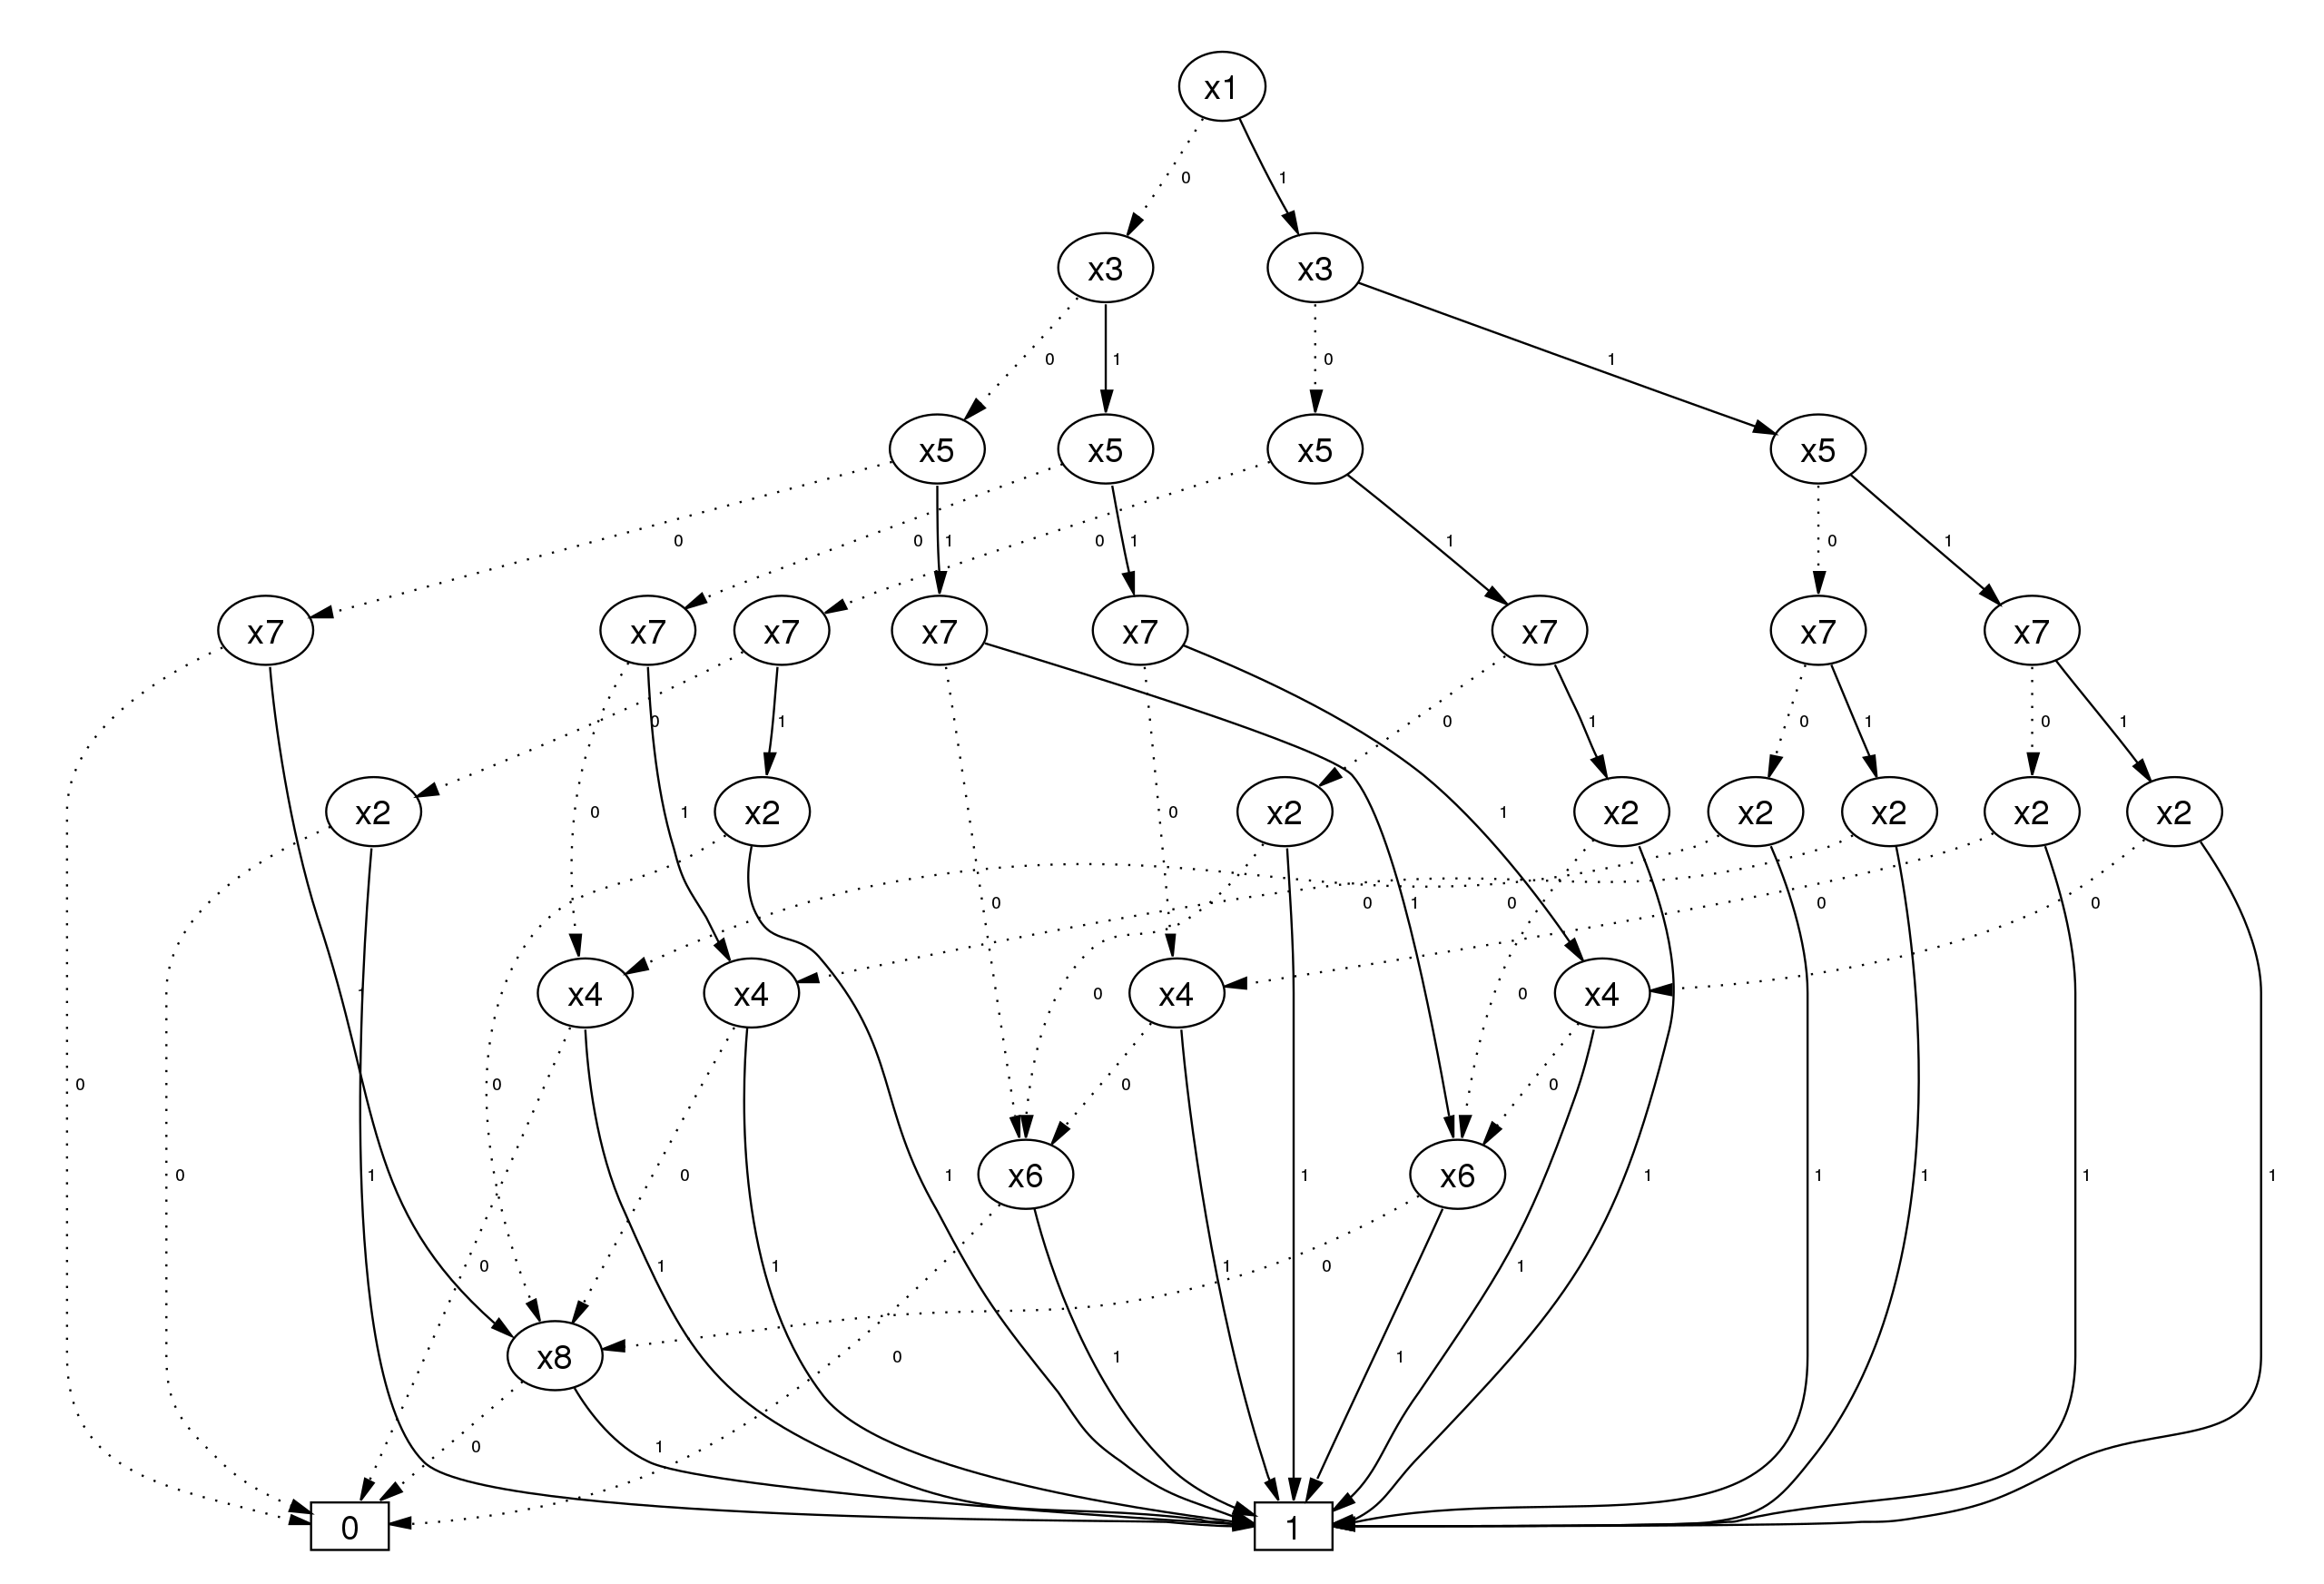
\includegraphics[height=6cm]{Img/BDD_Variable_Ordering_Bad.svg.pdf}
		\caption{索引顺序为\{x1,x3,x5,x7,x2,x4,x6,x8\}}
		\label{fig:bdd-bad}
	\end{subfigure}
    \qquad
	\begin{subfigure}[b]{.4\textwidth}
        \centering
        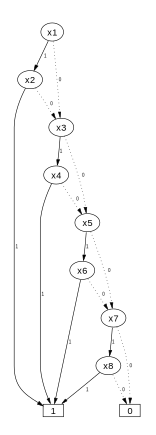
\includegraphics[height=6cm]{Img/BDD_Variable_Ordering_Good.svg.pdf}
		\caption{索引顺序为\{x1,x2,x3,x4,x5,x6,x7,x8\}}
		\label{fig:bdd-good}
	\end{subfigure}
	\caption{布尔函数$f (x1,...,x8)=x1x2+x3x4+x5x6+x7x8$在不同索引顺序下的BDD\citep{wiki:bdd}}
	\label{fig:bdd-compare}
\end{figure}

\section{软件系统实现}
为了实现软件的高效运行,模块化设计至关重要。
每个模块在软件系统中扮演着关键角色,并且具有特定的功能和目的。以下是本次毕业设计中软件必须包含的模块及其重要性的说明:
% //TODO: add more explain
\begin{itemize}
    \item \textbf{输入处理模块}:该模块的主要职责是处理输入数据,例如接收用OpenQASM格式编写的量子算法代码。其核心功能是将这些代码转换为TDD表示形式。鉴于当前存在多种量子编程语言,此模块的模块化处理能够显著提升系统的灵活性和兼容性。
    \item \textbf{内存管理模块}:本模块负责管理TDD节点的存储和维护。当创建新的TDD节点时,它会运用哈希算法与现有节点进行对比,以避免重复创建相同节点。这种方法不仅减少了内存占用,还提高了处理效率。
    \item \textbf{TDD基础模块}:该模块主要执行TDD节点的压缩操作,或者导出TDD的树状结构图。节点收缩是TDD核心的运算过程,而树状结构图的导出功能则有助于用户更好地理解和分析TDD的结构。
    \item \textbf{TDD算法模块}:此模块为TDD提供更复杂的算法支持。例如,它能够调整节点收缩的顺序,以优化系统运行效率。此外,它还能执行其他高级功能,如检验TDD是否存在于特定子空间中。
\end{itemize}
